Figure \ref{fig:the proposed approach} shows the proposed architecture to the ASL translator. The main approach to developing a translation from American SLA to other SLA is to build the best image recognition model that recognizes each American letter from the sign language with high accuracy. Instead of learning from scratch, transfer learning with pre-trained models, which were already trained on a large benchmark image dataset, can save a lot of computational cost and help the performance. Keras provides a wide range of pre-trained models for deep learning such as VGG, ResNet, Xception, etc \cite{keras}. All the available pre-trained models will be applied into the first run training with the partial dataset to find out the 5 best performing models from each architecture with the highest accuracy of prediction. The top 5 models will be further optimized and trained with all the training data to determine the most suitable ASL recognition model. In the last phase, the results of the prediction will be mapped with Turkish ASL images.

\begin{figure}[h]
    \centering
    \caption{The proposed approach for the sign language translator}
	\label{fig:the proposed approach}
    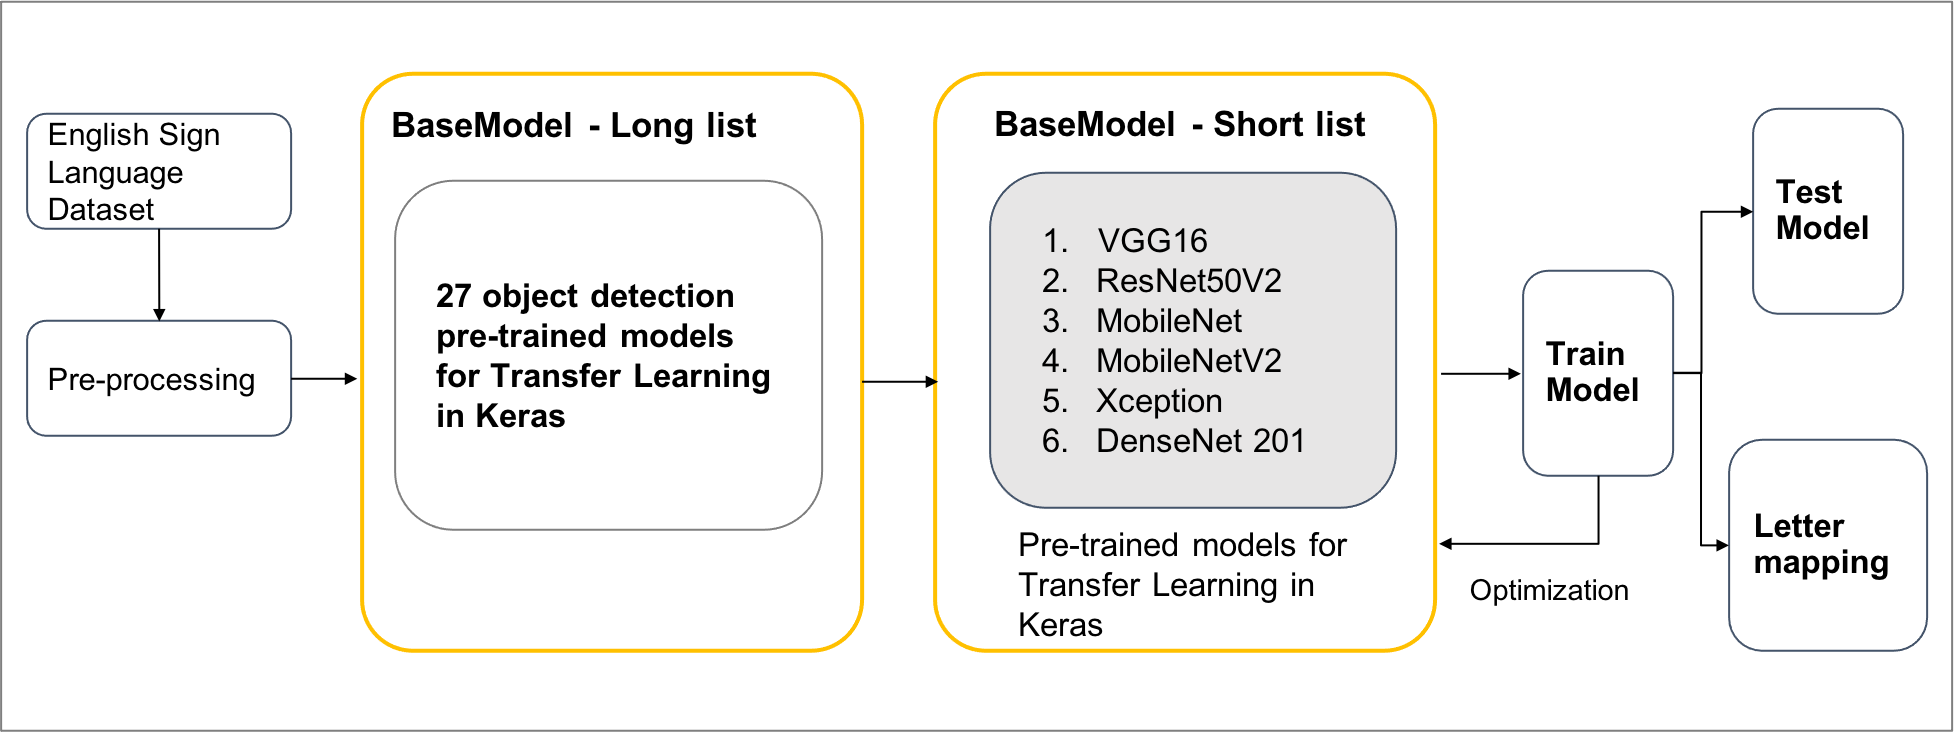
\includegraphics[width=\linewidth]{figures/The approach}
\end{figure}


\subsection{Dataset}
The American ASL dataset is collected from one of the top open-source dataset repositories, Kaggle. The dataset contains 87,000 images with 26 American letters and 3 extra signs, which are delete, space, and nothing. All the images are equally distributed to the 29 signs. In other words, each sign has 4,300 images. The whole dataset is split into training and test dataset. The training dataset is 80\% of the data, and the rest data belongs to the test dataset. 


\subsection{Image preprocessing}
The original image size in the dataset is 200 x 200 pixels, but the network of pre-trained models is trained on 224 x 224 color images. Therefore, the images in the dataset are then resized to 224 x 224 pixels and are at the same time randomly transformed with data augmentation by applying the Keras ImageDataGenerator class \cite{keras}. ImageDataGenerator class provides an ability to use data augmentation such as rotations, shift, brightness as well as zoom and return augmented images automatically when training a model to help improve model performance.

\subsection{Transfer learning models}\label{chapter_models}
One of the main benefits of using transfer learning is to make use of previously trained models and save computational cost (CC) for basic tasks like the removal of background. It may also be used when the training data is sparse. In transfer learning, the theory is that a model which has been trained for one purpose can easily be adapted to suit a different use case by transferring the learned knowledge to the other challenge\cite{zhuang2020comprehensive}. This is achieved by keeping the main structure and weights of the neural network and only changing the last layers to apply the way of classifying the final output. The lower layers, therefore, take care of more general tasks like identifying an object in an image\cite{neyshabur2021transferred} and the higher layers, the more specialised task. Not only does that enable the opportunity to achieve great results with only a small training dataset, but one also benefits from the big research field, which initially trains the model with more computational power. Transfer learning is especially applied in the field of computer vision, which is why it was chosen as a promising approach for the underlying research question.

For the detection of American SLA, we may use (to a degree) any pre-trained model for object detection on our dataset of American SLA signs even if they are limited in count and quality, as they only make the last layer of our final model.

To determine whether a model may be suitable for our application, we use all of the models and their variants available in Keras\cite{keras}, as shown in Table~\ref{tab:keras_models}. The \textit{Avg. Top-5 Accuracy} in the table refers to the average accuracy of all variants combined.
\begin{table}[th]
    \caption{Keras Applications}
    \label{tab:keras_models}
    \centering
    \begin{tabular}{@{}lrcl@{}}
    \toprule
    Name         & \multicolumn{1}{l}{\begin{tabular}[c]{@{}l@{}}Avg. Top-5\\ Accuracy\end{tabular}} & \multicolumn{1}{l}{Total} & \begin{tabular}[c]{@{}l@{}}Variants\\ (*=Model)\end{tabular}                         \\ \midrule
    Xception     & 0.945                                                                             & 1                         & *                                                                                    \\
    VGG          & 0.901                                                                             & 2                         & *16, *19                                                                             \\
    ResNet       & 0.931                                                                             & 6                         & \begin{tabular}[c]{@{}l@{}}*50, *101, *152,\\  *50V2, *101V2,\\  *152V2\end{tabular} \\
    Inception    & 0.945                                                                             & 2                         & *V3, *ResNetV2                                                                       \\
    MobileNet    & 0.898                                                                             & 2                         & *, *V2                                                                               \\
    DenseNet     & 0.930                                                                             & 3                         & *121, *169, *201                                                                     \\
    NASNet       & 0.940                                                                             & 2                         & *Mobile, *Large                                                                      \\
    EfficientNet & -                                                                                 & 8                         & \begin{tabular}[c]{@{}l@{}}*B0, *B1, *B2,\\  *B3, *B4, *B5,\\  *B6, *B7\end{tabular} \\ \bottomrule
    \end{tabular}
\end{table}

In order to define, which of the above stated models we will further evaluate and possibly optimize, we train each of the Keras models in an experimental setup. The experimental training is defined by:
\begin{enumerate}
    \item Training with 5\% of the dataset (4.300 images, equally distributed to the 29 targets), with an 80/20 Train-Test-Split
    \item 10 Epochs of Training
    \item No Early Stopping
\end{enumerate}

The results will focus on two key indicators: accuracy on our dataset and training time.

The following subsections will give a brief introduction of the most relevant model families and how they differ.

\subsubsection{VGG16}\label{chapter_vgg16}
The VGG models are one of the earlier computer vision models and were introduced in 2015 by Simonyan and Zisserman who showed that using deep architectures with rather small filters can be superior to other models at that time\cite{simonyan2015deep}. VGG represents a classical convolutional neural network that takes 224x224x3 (width x height x channels) input pictures and passes it to multiple convolutional layers, pooling layers and activation functions to a fully connected final layer for classification. It includes in total 16 layers with weights and is shown in figure \ref{fig:vgg16}.

\begin{figure}[ht]
  \centering
  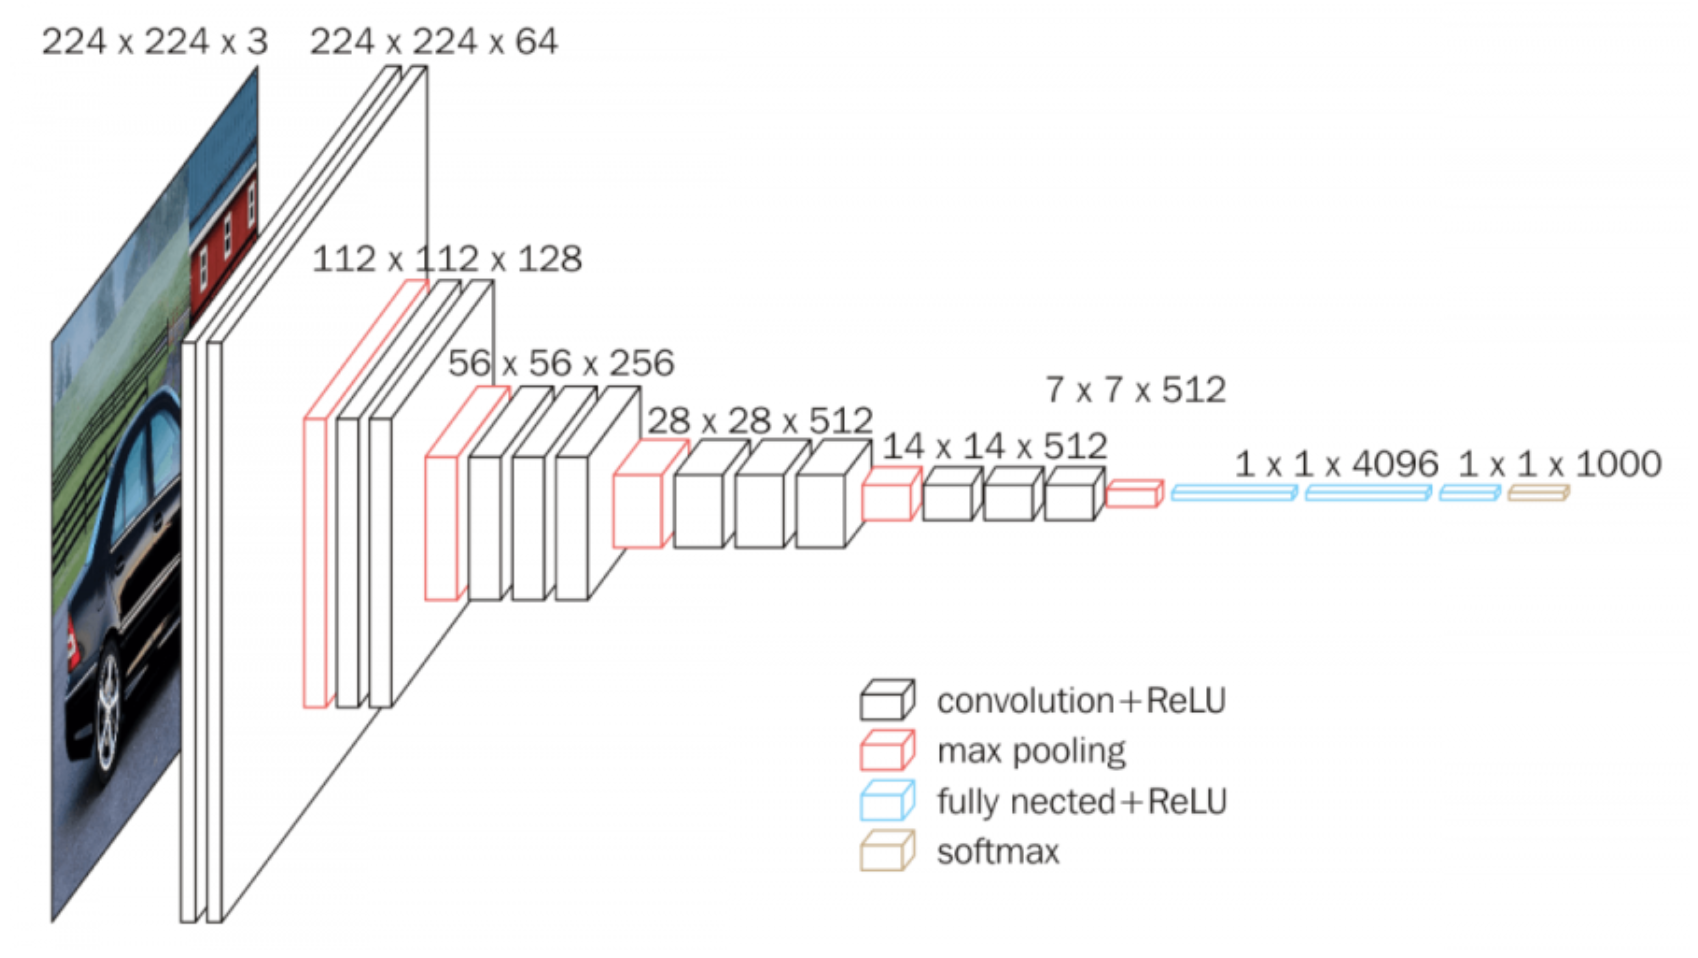
\includegraphics[width=\linewidth]{figures/vgg16.png}
  \caption{VGG16 architecture\cite{simonyan2015deep}}
  \label{fig:vgg16}
\end{figure}

The tremendous change compared to previous convolutional neural networks is that the used filters and layers have the same size and parameters such as only ReLu as activation function\cite{simonyan2015deep}. This newly introduced simplicity paired with a relatively deep architecture led to unique results in the ILSVRC-2012\ref{ILSVRC2012} and ILSVRC-2013\ref{ILSVRC2013} competitions compared to the previous state-of-art AlexNet. On top of that is was shown that the model had a strong ability to generalise over multiple datasets and still achieve a top 5 performance. The authors of the network structured it in a way that it is possible to move from 16 layers to 19 layers for even better results.

\subsubsection{ResNet50V2}\label{resnet}
Due to the fact that the performance of a very deep neural network started to decrease at some point, and the vanishing gradient while backpropagating became another problem, He et al. introduced the "residual units" for the new architecture\cite{he2015deep}. The main idea is to not only pass processed information from layer to layer but also to layers further ahead in the network. This skipping of e.g. one layer has been introduced as "skip-connection" or "identity shortcut." The layers and their connections to other layers are arranged as residual blocks which share the same input and output size within the block\cite{he2015deep}. The connection from one block to another is done by a "projection shortcut," which allows a change in input and output dimensions.

\begin{figure}[ht]
  \centering
  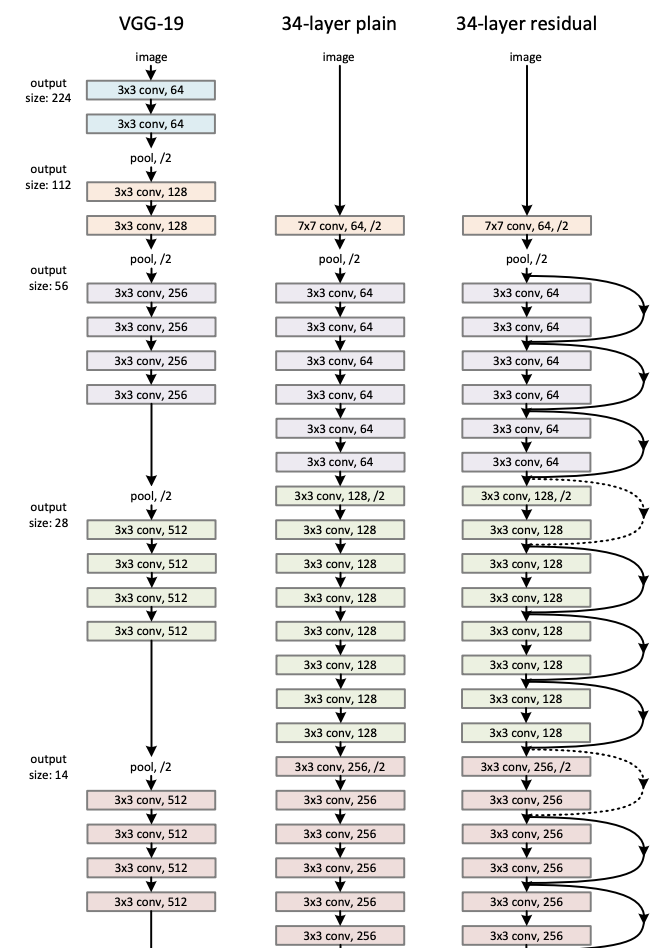
\includegraphics[width=\linewidth]{figures/resnet.png}
  \caption{ResNet architecture\cite{he2015deep}}
  \label{fig:resnet}
\end{figure}

Figure \ref{fig:resnet} presents the different residual units on the right side distinguished by the color. The dotted connections represent the projection shortcuts, whereas the solid arrows represent the identity shortcuts.
This newly introduced architecture enabled the authors to solve both of the above mentioned issues and build deep, high performing neural networks. The main reason for this achievement is that higher layers can learn important information from the lower layers directly.

\subsubsection{MobileNet}\label{mobilenet}

MobileNet was developed by Google Inc. with the purpose of being used for mobile and embedded vision applications. This target leads to the fact that the model has been optimised for latency.
The authors introduced "depthwise separable convolutions," in which the channels are separately convoluted on their own and only then combined through a 1x1 pointwise convolution\cite{howard2017mobilenets}. A visualisation can be found in figure \ref{fig:mobilenet}. This separation of the convolution for each channel and a followed combination of the feature map results in significantly less computation compared to the previous neural networks and therefore minimizes the latency drastically by approx. 8 times\cite{howard2017mobilenets}.

\begin{figure}[ht]
  \centering
  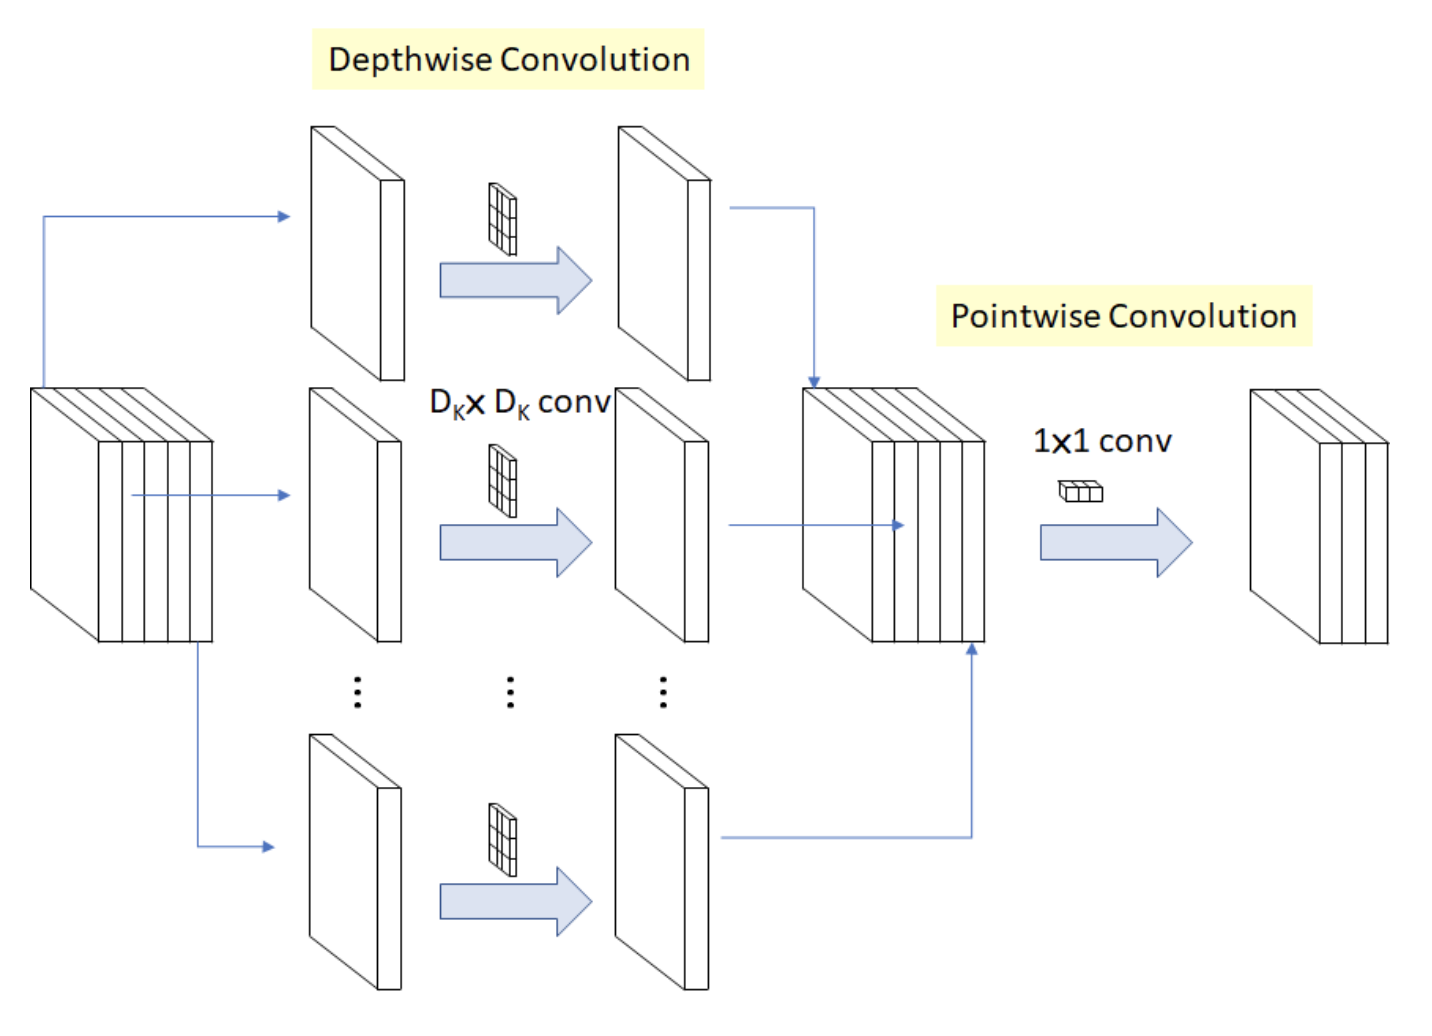
\includegraphics[width=\linewidth]{figures/mobilenet.png}
  \caption{MobileNet architecture\cite{howard2017mobilenets}}
  \label{fig:mobilenet}
\end{figure}

Besides the tremendous success with focus and latency such as high performance on the usual benchmark datasets for e.g. facial recognition, the authors found out that with this approach, less regularisation and data augmentation is needed to achieve state-of-the-art results.

\subsubsection{MobileNetV2}
The second version of the MobileNet introduces two additions to its predecessor. The first one is called the bottleneck layer, where a low-dimensional feature vector is passed to the respective layer, which then expands this vector to a high-dimensional space, applies a depthwise convolution and reduces the dimensions again to deliver the output\cite{sandler2019mobilenetv2}. This way, the number of computations through out the entire network is kept stable, which has a positive impact on the latency. As this technique leads to some loss of contained information, the authors introduced residual units which follow the same logic like the units explained in section \ref{resnet}. This way, information can be passed by skipping a layer and the information loss due to the bottleneck layer is reduced.

\begin{table}[th]
    \caption{MobileNet comparison}
    \label{tab:mobilenet_comparision}
    \centering
    \begin{tabular}{@{}lrcl@{}}
    \toprule
    Version         & \multicolumn{1}{l}{\begin{tabular}[c]{@{}l@{}}MACs (millions)\end{tabular}} & \multicolumn{1}{l}{Parameters (millions)}                        \\ \midrule
    MobileNetV1     & 569                                                                             & 4.24                                                                                 \\
    MobileNetV2          & 300                                                                             & 3.47\end{tabular}
\end{table}

\begin{table}[th]
    \caption{MobileNet FPS comparison}
    \label{tab:mobilenet_fps_comparision}
    \centering
    \begin{tabular}{@{}lrcl@{}}
    \toprule
    Version         & \multicolumn{1}{l}{\begin{tabular}[c]{@{}l@{}}iPhone 7\end{tabular}} & \multicolumn{1}{l}{iPhone X}& \multicolumn{1}{l}{iPad Pro 10.5}                        \\ \midrule
    MobileNetV1     & 118                                                                             & 162 & 204                                                                                \\
    MobileNetV2          & 145                                                                             & 233 & 220\end{tabular}
\end{table}

Additionally, the authors showed increased performance on benchmark datasets such as a potential combination with single shot detection (SSD), which can yield into even better and faster results.

\subsubsection{DenseNet 201}

Dense convolutional networks, also called DenseNet, were introduced in 2016 by Huang et al. and proposed a new way of building very deep neural networks which are stable to train and high performing. The change compared to other architectures was that each layer is connected to all following layers to pass the resulting feature vector through the entire network\cite{huang2018densely}. A visual illustration can be found in figure \ref{densnet}.

\begin{figure}[ht]
  \centering
  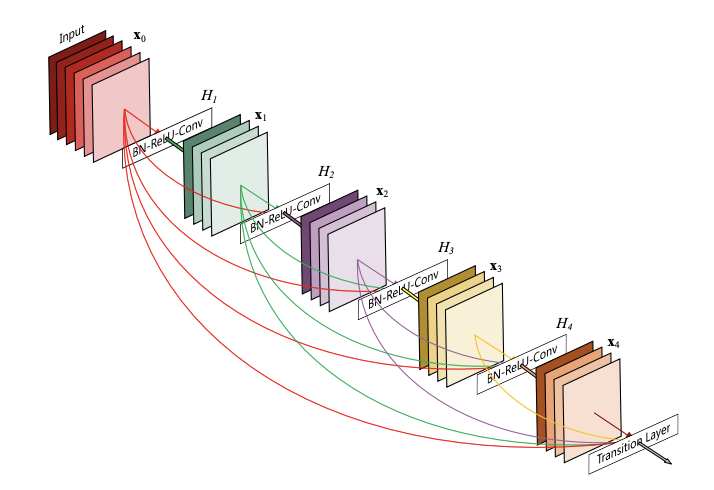
\includegraphics[width=\linewidth]{figures/densenet.png}
  \caption{DensNet architecture\cite{huang2018densely}}
  \label{densnet}
\end{figure}

The connection from one layer to all following layers is in a typical fast-forward manner which leads to the following advantages:
\begin{itemize}
  \item alleviate the vanishing-gradient problem
  \item stronger feature re-use
  \item smaller number of parameters
\end{itemize}

The reduced number of parameters is a result of the network being able to ignore redundant feature maps which do not need to be learned again. In the initial paper, the authors propose an architecture with very narrow layers (12 filters per layer)\cite{huang2018densely}. Due to the complete connection of all layers, the model is less likely to overfit and more stable to train.
The model contains residual units as well, which shall strengthen the information flow from previous to later layers. Additionally, bottleneck layers can be found, which were introduced to minimise the number of computations being caused by the complex connectivity.

\subsubsection{Xception}\label{chapter_xception}

Xception is an advanced version of Google's Inception model and a short form of "Extreme Inception". The previous architecture of Inception convoluted the input channel by channel and combined the results in the end. This depthwise separable convolution was slightly modified in the newly introduced Xception model by Chollet\cite{chollet2017xception}. The author changed the regular setup of first applying a depthwise convolution and then the pointwise to a setup that executes these steps the other way round. However, this change on its own did not lead to major improvements with regard to performance which is why a second change was applied by introducing residual connections\cite{chollet2017xception}.
\begin{figure}[ht]
  \centering
  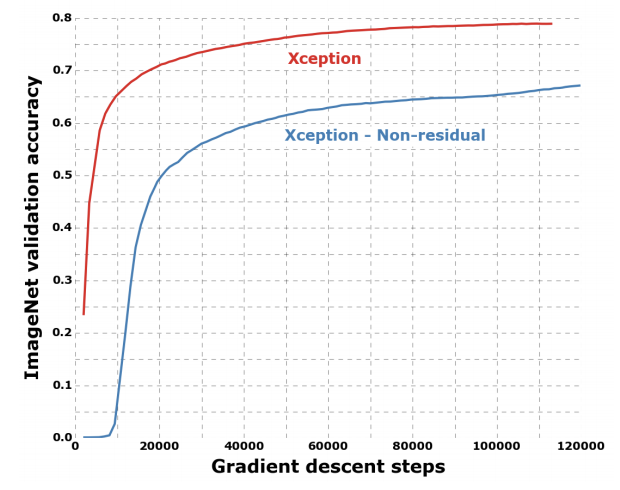
\includegraphics[width=\linewidth]{figures/xception_residuals.png}
  \caption{Impact of residual units for Xception\cite{chollet2017xception}}
  \label{xception_residuals}
\end{figure}

Figure \ref{xception_residuals} shows a clear improvement of the introduction of residual blocks.

Furthermore, the author removed the ReLu activation after the depthwise convolution, different than in the Inception architecture, which had a tremendous impact on the model performance.
\begin{figure}
  \centering
  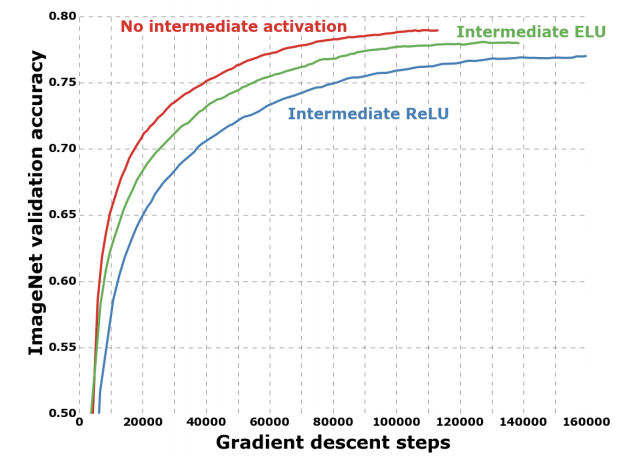
\includegraphics[width=\linewidth]{figures/xception_activation.png}
  \caption{Impact of removing ReLu activation\cite{chollet2017xception}}
  \label{xception_activation}
\end{figure}

The changes not only led to a similar model size like Inception-V3 but also outperformed  VGGNet, ResNet, and Inception-V3 in accuracy with regard to known benchmark datasets\cite{chollet2017xception}.

\subsection{Evaluation metric}

The following evaluation will use the model accuracy as a final metric to define  each model's performance. The accuracy will be calculated for each target variable and then averaged over all classes. The calculation can be described as:
\begin{equation}
ACC=\frac{1}{N} \sum_\textit{i=1}^{N_\textit{c}} \displaystyle\frac{TP_{\textit{i}}+TN_{\textit{i}}}{TP_{\textit{i}}+TN_{\textit{i}}+FP_{\textit{i}}+FN_{\textit{i}}}
\end{equation}
\break
$N_\textit{c}=\textit{Number of classes}$\\
$TP_\textit{i} = \textit{Count of true positive predictions for given class}$\\
$TN_\textit{i} = \textit{Count of true negative predictions for given class}$\\
$FP_\textit{i} = \textit{Count of false positive predictions for given class}$\\
$FN_\textit{i} = \textit{Count of false negative predictions for given class}$





